% ICASSP 2027 draft. The official 2027 author kit was not linked from the
% conference site on 2026-08-19; this uses the official ICASSP 2026 spconf
% layout and must be checked against the 2027 kit before submission.
\documentclass{article}
\usepackage{spconf}
\usepackage{booktabs}
\usepackage{graphicx}
\usepackage{hyperref}
\title{When Cautious Template Memory Hurts: A Reproducible\
Training-Free Study of Frozen FARTrackSparse}
\name{Anonymous Authors}
\address{Anonymous Affiliation}

\begin{document}
\ninept
\maketitle
\begin{keywords}
Visual object tracking, template memory, autoregressive tracking, negative results, reproducibility.
\end{keywords}

\begin{abstract}
Template updates make visual trackers adapt to changing appearance, but can also
propagate a localization error.  We conduct a controlled, training-free study
of five memory interventions for a frozen FARTrackSparse checkpoint.  The
development protocol uses the public GOT-10k validation set (180 sequences,
21,007 frames), while full LaSOT Testing is held out until configuration
freezing.  Three complete development evaluations show that hard write holding,
counterfactual write rejection, and stable-anchor recovery reduce mean frame
IoU by 0.00823, 0.02000, and 0.03204, respectively, relative to the immutable
baseline.  Two soft rebinding variants fail fixed-screen directionality or
efficiency gates.  Thus no proposed intervention is claimed as an improvement.
The contribution of this draft is a transparent negative-result record,
including checked implementation failures, statistical uncertainty, and a
reproducible protocol. The frozen baseline-only LaSOT reference gives a local
success AUC of 0.6148 on 280 Protocol-II sequences; no rejected candidate was
run on that held-out set.
\end{abstract}

\section{Introduction}
Autoregressive tracking exposes a practical tension: recent templates improve
adaptation, while an erroneous crop may contaminate later predictions. FARTrack
uses autoregression and inter-frame sparsification to obtain fast tracking
\cite{wang2026fartrack}.  We asked a deliberately narrow question: can
untrained control of its inference-time template memory improve a released,
frozen FARTrackSparse checkpoint without additional training?

This paper reports the answer for the mechanisms tested: no.  We regard this
as useful evidence because plausible memory protections can silently damage the
update distribution expected by a frozen tracker.  We do not replace this
negative result with a post-hoc positive claim.

\section{Protocol}
\noindent\textbf{Model and invariants.} Every experiment uses the released
\texttt{FARTrackSparse\_ep0015.pth.tar} checkpoint, the original prediction
decoder, the original result writer, and the same initialization boxes. The
baseline tracker is exposed as \texttt{fartrack\_sparse\_research}; its
upstream inference implementation is not modified.

\noindent\textbf{Development/test separation.} B\textsubscript{dev} is the public
GOT-10k validation split. GOT-10k was introduced as a high-diversity generic
tracking benchmark with an explicit one-shot protocol \cite{huang2021got10k}.
The development metric is mean frame IoU (AO) over 180 sequences and 21,007
frames, calculated by a read-only local script which checks sequence coverage
and prediction lengths. Full official LaSOT Testing is B\textsubscript{test}.
LaSOT supplies dense, long sequences for SOT evaluation \cite{fan2019lasot}.
It was checksum-verified and not accessed until all candidate decisions were
frozen. The B\textsubscript{test} run is baseline-only because no candidate
survived B\textsubscript{dev}. It measured success AUC 0.6148, precision at
20 pixels 0.6446, and normalized precision AUC 0.6399. This is an external
baseline reference, not a new-method result; no cross-run comparison to
upstream repository tables is claimed.

\noindent\textbf{Statistics and speed.} We report the mean of per-frame IoUs. For a
candidate-baseline comparison, we resample the 180 per-sequence AO differences
10,000 times with seed 20260819 and report a percentile 95\% interval. Aggregate
FPS is total frames divided by the sum of saved per-frame times. These intervals
describe the observed development set; they are not independent-video
population inference.

\section{Interventions}
\begin{enumerate}
  \item \textbf{TRM-FAR}: a transaction ledger holds writes under three causal
  anomaly signals and rolls back after sustained failure.
  \item \textbf{Counterfactual agreement}: old-only and recent-only template
  views gate a write when their coordinate predictions disagree. It requires
  two extra forwards after warm-up.
  \item \textbf{Stable-anchor recovery}: persistent failures temporarily replay
  the initial template and the last accepted view.
  \item \textbf{Recent-consensus rebinding}: all frames are written, but fixed
  template slots are rebound using untrained RGB descriptor medoids.
  \item \textbf{Appearance-diverse rebinding}: all frames are written, while
  slots retain chronological max--min RGB descriptor exemplars.
\end{enumerate}

All implementations are separate tracker entry points. Focused unit tests and
GPU smoke tests preceded evaluation. Counterfactual agreement initially exposed
an out-of-range indexing defect after a rejected write; it was repaired by
indexing its bounded template pool by accepted writes, and only the repaired
version was evaluated.

\section{Results}
\begin{table}[h]
\centering
\caption{Complete B\textsubscript{dev} results. AO is mean frame IoU.}
\begin{tabular}{lrrrr}
\toprule
Method & AO & $\Delta$ AO & 95\% paired interval & FPS \\
\midrule
Immutable FARTrackSparse & 0.832741 & 0.000000 & -- & 40.07 \\
TRM-FAR & 0.822471 & -0.008228 & [-0.019499, 0.004104] & 42.16 \\
Counterfactual agreement & 0.806470 & -0.019995 & [-0.037073, -0.003256] & 23.47 \\
Stable-anchor recovery & 0.797473 & -0.032038 & [-0.050311, -0.015034] & 40.90 \\
Logarithmic sampler & 0.830650 & -0.002730 & [-0.010716, 0.003984] & 31.32 \\
\bottomrule
\end{tabular}
\end{table}

\begin{figure}[h]
\centering
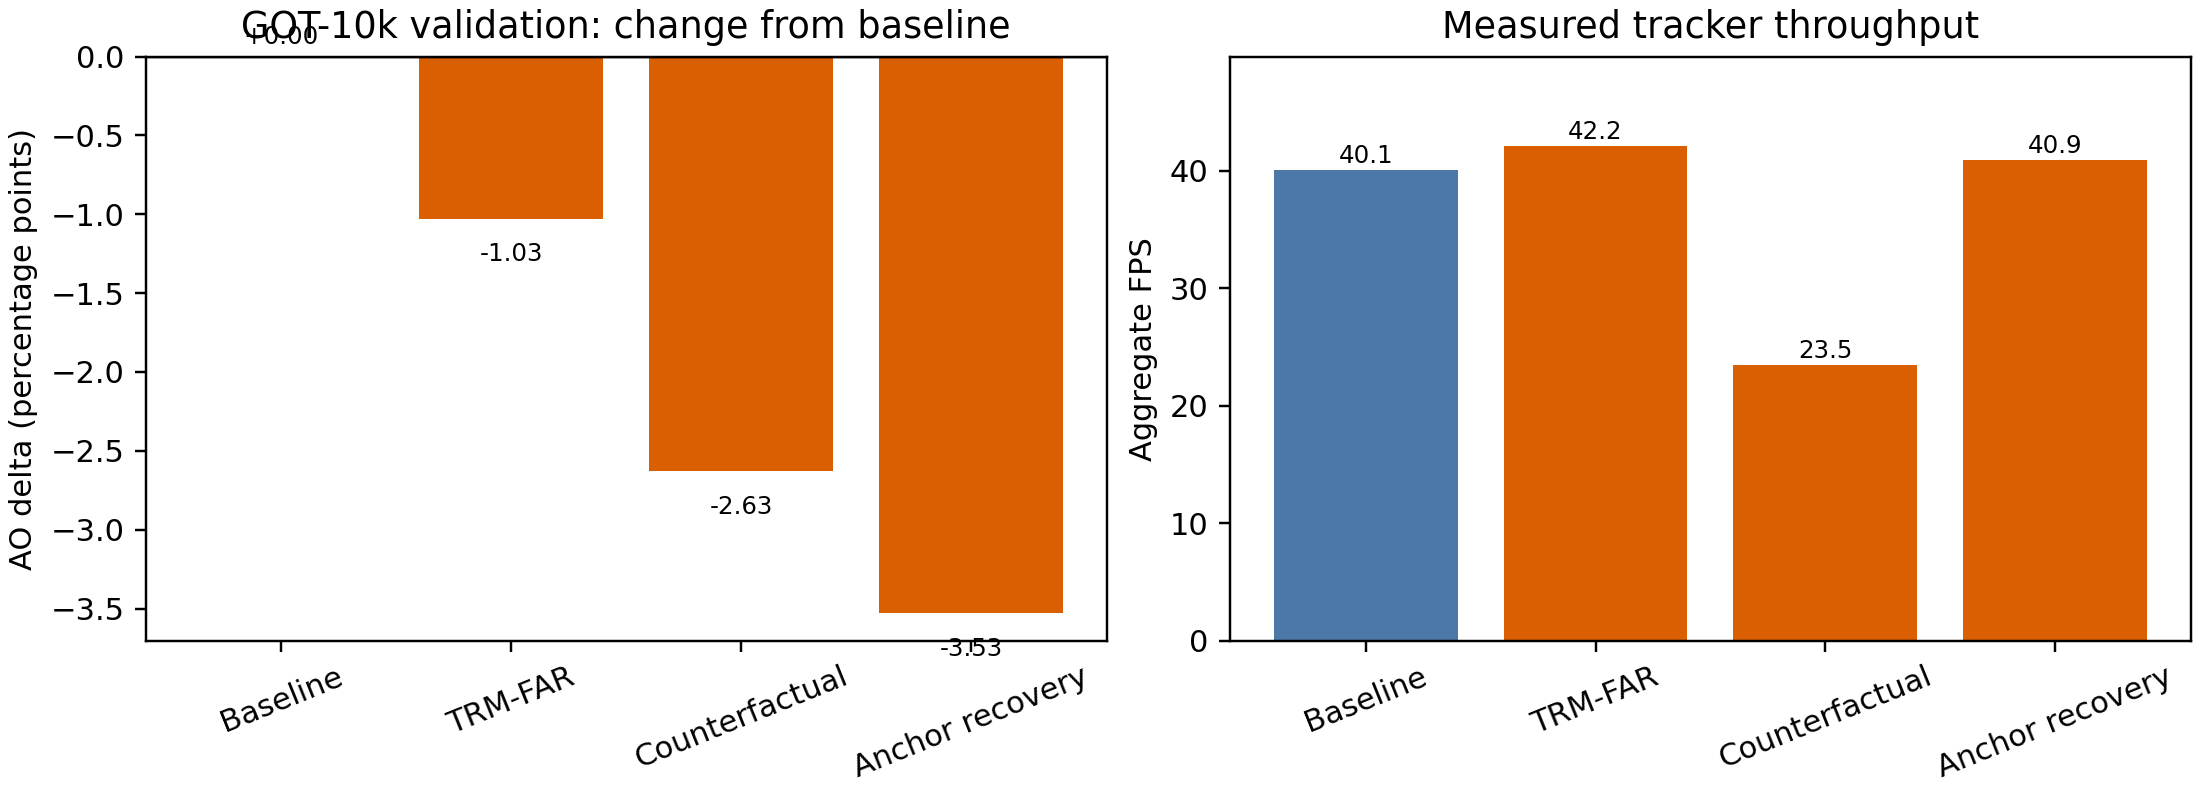
\includegraphics[width=\linewidth]{../figures/got10k_bdev_memory_interventions.png}
\caption{Measured complete GOT-10k validation outcomes. Orange bars are
rejected candidate mechanisms; the graphic reports observed B\textsubscript{dev}
data only and is not a held-out benchmark result.}
\end{figure}

TRM-FAR improved 70 sequences and degraded 110; stable-anchor recovery improved
66 and degraded 114; counterfactual agreement improved 77 and degraded 103.
No candidate in Table~1 was tuned after its complete development result or run
on B\textsubscript{test}.

The two soft alternatives did not pass their prespecified focused-screen gates.
Recent-consensus rebinding obtained 0.907830 versus 0.909803 for the baseline
on a fixed 60-frame screen. Appearance-diverse rebinding obtained a small
0.000838 AO increase on a fixed 80-frame screen, but incurred a 16.57\% FPS
loss (21.93 versus 26.28 FPS), exceeding the 5\% gate. These are screening
observations, not generalization estimates, and were not expanded to a full
development evaluation.

\section{Discussion and Limitations}
The shared pattern is that hard intervention can sacrifice normal appearance
adaptation more often than it prevents memory pollution. Uncertainty, motion
inconsistency, and disagreement are not calibrated error probabilities for a
frozen model. Further, changing the effective template distribution may create
an input regime unseen during training. This study does not establish that
template control is never useful; it only rejects these implementations and
fixed settings on the stated protocol.

Limitations are substantial. There is one released checkpoint, one full public
development split, RGB descriptors rather than learned confidence, and no
positive method. The LaSOT outcome is a baseline-only reference; it cannot
validate a rejected candidate. GOT-10k test server submission has not been
performed.

\section{Reproducibility and Disclosure}
All source changes, commands, structured metrics, logs, and immutable checkpoint
path are documented in \texttt{research/EXPERIMENT\_LOG.md}. Data archives and
outputs reside on the data disk. This draft was prepared with AI assistance;
human authors must verify all text, select authorship, and approve any
submission. No funding, conflict-of-interest, or authorship statements are
asserted because they were not provided.

\bibliographystyle{IEEEbib}
\bibliography{references}
\end{document}
